 \let\negmedspace\undefined
\let\negthickspace\undefined
\documentclass[journal]{IEEEtran}
\usepackage[a5paper, margin=10mm, onecolumn]{geometry}
%\usepackage{lmodern} % Ensure lmodern is loaded for pdflatex
\usepackage{tfrupee} % Include tfrupee package

\setlength{\headheight}{1cm} % Set the height of the header box
\setlength{\headsep}{0mm}     % Set the distance between the header box and the top of the text
\usepackage{gvv-book}
\usepackage{gvv}
\usepackage{cite}
\usepackage{amsmath,amssymb,amsfonts,amsthm}
\usepackage{algorithmic}
\usepackage{graphicx}
\usepackage{textcomp}
\usepackage{xcolor}
\usepackage{txfonts}
\usepackage{listings}
\usepackage{enumitem}
\usepackage{mathtools}
\usepackage{gensymb}
\usepackage{comment}
\usepackage[breaklinks=true]{hyperref}
\usepackage{tkz-euclide} 
\usepackage{listings}
% \usepackage{gvv}                                        
\def\inputGnumericTable{}                                 
\usepackage[latin1]{inputenc}                                
\usepackage{color}                                            
\usepackage{array}                                            
\usepackage{longtable}                                       
\usepackage{calc}                                             
\usepackage{multirow}                                         
\usepackage{hhline}                                           
\usepackage{ifthen}                                           
\usepackage{lscape}



\usepackage{amsmath,amssymb}
\usepackage{booktabs}
\usepackage{tikz}
\usetikzlibrary{arrows.meta,angles,quotes}





\begin{document}

\bibliographystyle{IEEEtran}
\vspace{3cm}

\title{2.10.10}
\author{AI25BTECH11021 - Abhiram Reddy N}
% \maketitle
% \newpage
% \bigskip
{\let\newpage\relax\maketitle}

\renewcommand{\thefigure}{\theenumi}
\renewcommand{\thetable}{\theenumi}
\setlength{\intextsep}{10pt} % Space between text and floats


\numberwithin{equation}{enumi}
\numberwithin{figure}{enumi}
\renewcommand{\thetable}{\theenumi}


\section*{Question}

Given that
\[
\mathbf{a} = \begin{pmatrix} 1 \\ 1 \\ 1 \end{pmatrix}, \quad
\mathbf{c} = \begin{pmatrix} 0 \\ 1 \\ -1 \end{pmatrix}, \quad
\mathbf{a} \cdot \mathbf{b} = 3, \quad
\mathbf{a} \times \mathbf{b} = \mathbf{c},
\]
find \(\mathbf{b}\).

\section*{Solution}

\subsection*{Step 1: Express vectors as column matrices}

\[
\mathbf{a} = \begin{pmatrix} 1 \\ 1 \\ 1 \end{pmatrix}, \quad
\mathbf{b} = \begin{pmatrix} x \\ y \\ z \end{pmatrix}, \quad
\mathbf{c} = \begin{pmatrix} 0 \\ 1 \\ -1 \end{pmatrix}.
\]

\subsection*{Step 2: Use the dot product condition}

\[
\mathbf{a}^\top \mathbf{b} = x + y + z = 3.
\]

\subsection*{Step 3: Use the cross product condition}

\[
\mathbf{a} \times \mathbf{b} = 
\begin{pmatrix}
z - y \\
x - z \\
y - x
\end{pmatrix}
= 
\begin{pmatrix}
0 \\
1 \\
-1
\end{pmatrix}.
\]

From which we get:
\[
\begin{cases}
z - y = 0, \\
x - z = 1, \\
y - x = -1.
\end{cases}
\]

\subsection*{Step 4: Solve the system}

From \(z - y = 0\), we have
\[
z = y.
\]

From \(y - x = -1\), we get
\[
y = x - 1.
\]

Substitute into \(x - z = 1\) (with \(z = y\)):
\[
x - y = 1 \implies x - (x - 1) = 1 \implies 1 = 1,
\]
which is consistent.

\subsection*{Step 5: Use the dot product to find \(x\)}

\[
x + y + z = x + (x - 1) + (x - 1) = 3x - 2 = 3 \implies 3x = 5 \implies x = \frac{5}{3}.
\]

Then,
\[
y = \frac{2}{3}, \quad z = \frac{2}{3}.
\]

\subsection*{Final answer}

\[
\boxed{
\mathbf{b} = \begin{pmatrix} \frac{5}{3} \\[6pt] \frac{2}{3} \\[6pt] \frac{2}{3} \end{pmatrix}.
}
\]





\begin{figure}[htbp]
\centering
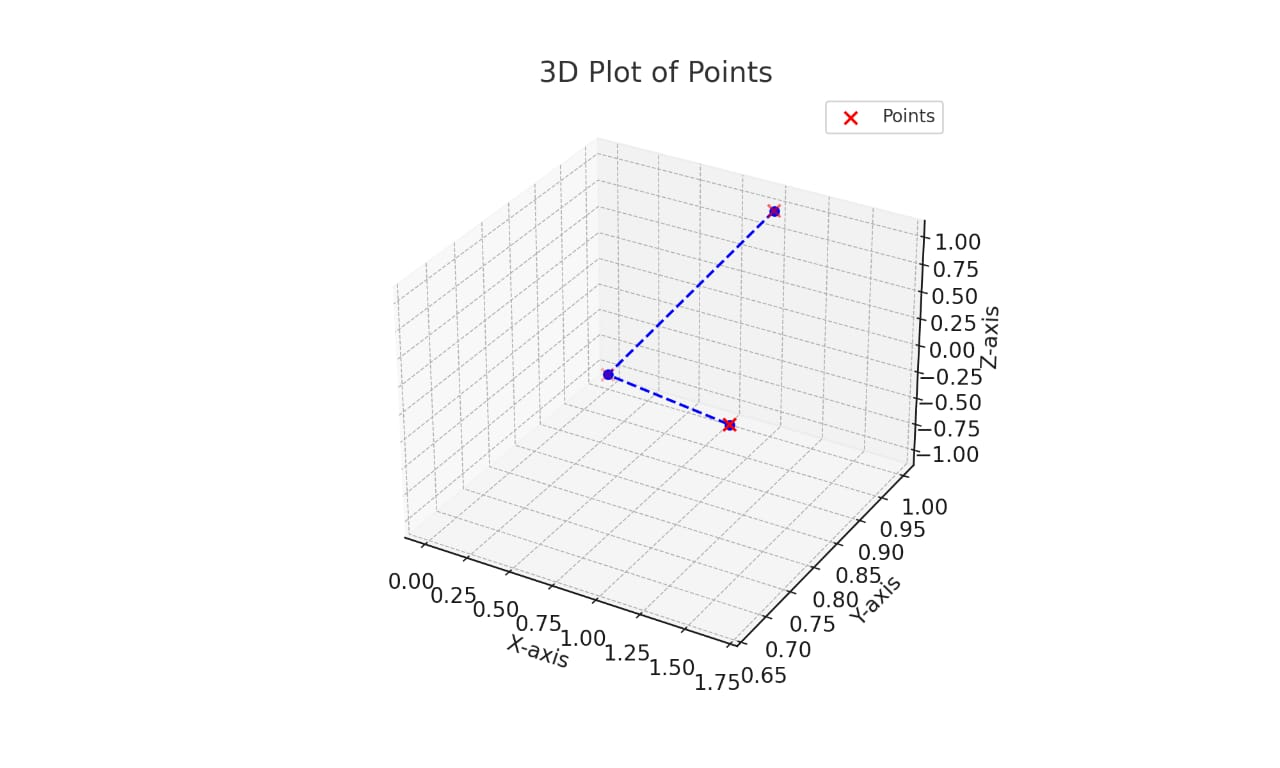
\includegraphics[width=\columnwidth]{figs/python_plot.png} 
\caption{plot}
\label{fig:1}
\end{figure}



\end{document}